\MonsterSheetGeometry

% --------------------------------------------------------------------------------------------------- %
% ################################################################################################### %
% #-#-#-#-#-#-#-#-#-#-#-#-#-#-#-#-# Monster-Sheet  with full Footer #-#-#-#-#-#-#-#-#-#-#-#-#-#-#-#-# %
% ################################################################################################### %
% --------------------------------------------------------------------------------------------------- %

\MonsterFooterGraphic{175pt}{430pt}{Monsters/Cobalt_Fox.png}{}
\addImageDBEntry{CobaltFox1}{Page \thepage}{Art}{https://www.artofmtg.com/art/flourishing-fox/}{Flourishing Fox MtG Art from Ikoria}{Ilse Gort}%

% Monster stat block
\vspace*{-2.75cm}\begin{DndMonster}[width=0.5\textwidth]{Cobalt Fox\label{monster:CobaltFox}}
    \DndMonsterType{Small Fey, chaotic good}

    % If you want to use commas in the key values, enclose the values in braces.
    \DndMonsterBasics[
        armor-class = {12},
        hit-points  = {\DndDice{6d6 + 4}},
        speed       = {40 ft., burrow 10 ft.},
        initiative	= {+4},
    ]

    \DndMonsterAbilityScores[
        str = 8,
        dex = 18,
        con = 9,
        int = 12,
        wis = 16,
        cha = 14,
    ]

    \DndMonsterDetails[
        saving-throws = {Dex +7, Int +5, Cha +5},
        skills = {Perception +4, Stealth +7},
        %damage-vulnerabilities = {cold},
        %damage-resistances = {bludgeoning, piercing, and slashing from nonmagical attacks},
        %damage-immunities = {cold},
        senses = {Darksight 60ft., Passive Perception 14},
        %condition-immunities = {frightened, poisoned},
        languages = {Sylvan},
        challenge = 2,
    ]
    
	\DndMonsterAction{Fearsome Agility}
	The Cobalt Fox can take the Dash Action as a Bonus Action. Also, Cobalt Foxes do not trigger opportunity attacks.    
	
	\DndMonsterAction{Keen Hearing and Smell}
	The Cobalt Fox has advantage on Perception checks that rely on hearing or smell.
	
	\DndMonsterAction{Innate Spellcasting}
	The Cobalt Fox can innately cast the following spells, without any components. Its spellcasting ability is Wisdom (spell save DC 14):
	\begin{itemize}
		\item At will: Aid, Cure Wounds
		\item 2/day: Beacon of Hope, Blink
		\item 1/day: Alter Self, Dispel Magic
	\end{itemize}
	
	\DndMonsterAction{Ventriloquism}
	The Cobalt Fox can make its bark (or any sound that it can make) seem to issue from someplace else. With respect to such voices and sounds, anyone who hears the sound can attempt a DC 14 Intelligence (Investigation) check. On success, they recognize it as illusory but still hear it.
    
    \DndMonsterSection{Actions}	
	\DndMonsterAttack[
      name=Bite,
      distance=melee, % valid options are in the set {both,melee,ranged},
      %type=weapon, %valid options are in the set {weapon,spell}
      mod=+2,
      reach=5,
      %range=20/60,
      targets=one target,
      dmg=\DndDice{2d4 + 2},
      dmg-type=piercing,
      %plus-dmg=,
      %plus-dmg-type=,
      %or-dmg=,
      %or-dmg-when=,
      %extra=,
    ]
    
    \DndMonsterAttack[
      name=Gore,
      distance=melee, % valid options are in the set {both,melee,ranged},
      %type=weapon, %valid options are in the set {weapon,spell}
      mod=+4,
      reach=5,
      %range=20/60,
      targets=one target,
      dmg=\DndDice{2d6 + 2},
      dmg-type=piercing,
      %plus-dmg=,
      %plus-dmg-type=,
      %or-dmg=,
      %or-dmg-when=,
      %extra=,
    ]
    
    \DndMonsterAction{Chromatic Burst}
    The fox creates a burst of flickering lights targeting a creature within 30ft. of it. The target must succeed on a DC 13 Wisdom saving throw. On a failed save the target takes \DndDice{2d10 + 4} radiant damage and is blinded until the start of the fox's next turn.
      
\end{DndMonster}

\vfill\eject

\nopagebreakchapter{\hspace*{\columnwidth + 20pt}Cobalt Fox}\phantomsection\addcontentsline{toc}{section}{Cobalt Fox}
\vspace*{-6\fontdimen6\font}

\entryfont \noindent \DndDropCapLine{B}looming flower meadows and an abundance of translucent red crystals sprout from the ground. Experienced travellers know they stepped into the territory of Cobalt Foxes. These elusive and magical creatures are distinguished by their dominant gem horn, indistinguishable from the ones spreading throughout their Lair. Although considered a creature of Feywild, they often build their burrows on the Material Plane offering other fey creatures a habitat of their liking.

\DndMonsterAction{Playful but Territorial} The Cobalt Fox itself is appraised as a very intelligent and often supportive fey helping other creatures and humanoids to find there way back to civilization or crucial infrastructure as well as towards feeding and drinking grounds. However, these creature can get highly aggressive and territorial if they sense harm towards their lair and are considered extremely ferocious if their cubs are in danger.\\

\subsection*{Cobalt Fox Lairs}
The presence of this fey fox has an effect on the wilderness around it. The flowers and vegetation is flourishing and seem more vibrant and give off a very strong fragrance. Additionally, small red crystals, so called "fox gems" or "foxes' jewels" are rising up throughout its territory. Not much is known about these crystals, nevertheless a really strong relationship between it and the abilities of Cobalt \linebreak

% --------------------------------------------------------------------------------------------------- %
% ################################################################################################### %
% #-#-#-#-#-#-#-#-#-#-#-#-#-#-# Monster-Sheet with  full Banner-Graphic #-#-#-#-#-#-#-#-#-#-#-#-#-#-# %
% ################################################################################################### %
% --------------------------------------------------------------------------------------------------- %

\MonsterBannerGraphic%
	{}% name of the monster to be displayed as header
	{section}
	{250pt}% offset for the section header
	{0pt} % Move Header horizontally
	{0pt} % Move Header vertically
	{300pt}% max height of the image
	{Monsters/Cobalt_Fox_Lair.png}% image to be displayed as a banner
	{}% used for keepaspectratio for image ({} or {, keepaspectratio})
	
\addImageDBEntry{CobaltFox2}{Page \thepage}{Background Art}{https://www.artofmtg.com/art/bloodfell-caves-3/}{Bloodfell Caves MtG Art from Ikoria}{Titus Lunter}%
	
\noindent Foxes cannot be denied. Studying these crystals turns out to be difficult as they are fiercely defended by the foxes protecting them like their own cub. Therefore, these stones are considered a very coveted magical item.\\
If a pair of Cobalt Foxes build their lair and birth cubs, the territory gets the following Lair Actions.

\subsection*{Lair Actions}
On initiative count 20, any Cobalt Fox considered to be part of the territory takes a lair action to cause one of the following effect. The same effect cannot be used two rounds in a row:
\begin{itemize}
	\item A "fox gem" creates a burst of flickering lights targeting a creature within 10ft. of it. The target must succeed on a DC 12 Wisdom saving throw. On a failed save the target takes \DndDice{1d10} radiant damage and is blinded until the start of the fox's next turn.
	\item A Cobalt Fox within 5ft. of a "fox gem" moves within 5ft. of another "fox gem".
	\item The "fox gem" starts to shimmer. Any creature that isn't a Cobalt Fox has disadvantage on Wisdom and Charisma saving throws until the end of the fox's next turn.
	\item The Zircon Fox can target \DndDice{1d8 + 1} "fox gems" it can see, teleporting to one of them and creating illusions of itself at the others. The illusions have 1 hitpoint and do not make any damage. \textbf{(Only Zircon Fox; 1/Day)}
\end{itemize}

\subsection*{Regional Effects}
The presence of the Cobalt Fox's lair has a slow but steady effect on its surroundings, creating one or more of the following effects:
\begin{itemize}
	\item \textbf{Crystal Profusion.} Natural stone within 500 feet of the lair grows plentiful crystal formations, known as "fox gems".
	\item \textbf{Beautiful Flora.} Flowers and other plants within a 3 miles radius of the lair look especially vibrant and beautiful.
	\item \textbf{Peaceful Atmosphere.} Fey creatures and creatures with fey ancestry within 3 miles of the lair are more at ease and are thus more abundant in the area.
\end{itemize}
If all the Cobalt Foxes die or leave the area, the effects fade over the course of \DndDice{1d10} days.

\vfill\eject

% Monster stat block
\vspace*{-130pt}\begin{DndMonster}[width=0.5\textwidth +0.5em]{Zircon Fox\label{monster:ZirconFox}}
    \DndMonsterType{Small Fey, chaotic evil}

    % If you want to use commas in the key values, enclose the values in braces.
    \DndMonsterBasics[
        armor-class = {16},
        hit-points  = {\DndDice{14d6 + 10}},
        speed       = {40 ft., burrow 10 ft.},
        initiative	= {+9},
    ]

    \DndMonsterAbilityScores[
        str = 14,
        dex = 20,
        con = 12,
        int = 14,
        wis = 14,
        cha = 8,
    ]

    \DndMonsterDetails[
        saving-throws = {Dex +9, Int +6},
        skills = {Perception +6, Stealth +9},
        %damage-vulnerabilities = {cold},
        %damage-resistances = {bludgeoning, piercing, and slashing from nonmagical attacks},
        %damage-immunities = {cold},
        senses = {Darksight 60ft., Passive Perception 14},
        %condition-immunities = {frightened, poisoned},
        languages = {Sylvan},
        challenge = 6,
    ]
    
	\DndMonsterAction{Fearsome Agility}
	The Zircon Fox can take the Dash Action or an Attack Action as a Bonus Action. It does not trigger opportunity attacks.
	
	\DndMonsterAction{Innate Spellcasting}
	The Zircon Fox can innately cast the following spells, without any components. Its spellcasting ability is Wisdom (spell save DC 16):
	\begin{itemize}
		\item At will: Bane, Blur
		\item 3/day: Dispel Magic, Chaos Bolt
		\item 1/day: Antilife Shell, Circle of Death
	\end{itemize}
    
    \DndMonsterSection{Actions}	
	\DndMonsterAttack[
      name=Bite,
      distance=melee, % valid options are in the set {both,melee,ranged},
      %type=weapon, %valid options are in the set {weapon,spell}
      mod=+4,
      reach=5,
      %range=20/60,
      targets=one target,
      dmg=\DndDice{3d8 + 5},
      dmg-type=piercing,
      %plus-dmg=,
      %plus-dmg-type=,
      %or-dmg=,
      %or-dmg-when=,
      %extra=,
    ]
    
    \DndMonsterAttack[
      name=Gore,
      distance=melee, % valid options are in the set {both,melee,ranged},
      %type=weapon, %valid options are in the set {weapon,spell}
      mod=+6,
      reach=5,
      %range=20/60,
      targets=one target,
      dmg=\DndDice{3d10 + 3},
      dmg-type=piercing,
      %plus-dmg=,
      %plus-dmg-type=,
      %or-dmg=,
      %or-dmg-when=,
      extra={. The target must succeed a DC 16 Constitution throw. On a fail the target bleeds},
    ]
    
    \DndMonsterAction{Achromatic Burst}
    The Zircon Fox creates an aura of darkness targeting a creature within 30ft. of it. The target must succeed on a DC 15 Wisdom saving throw. On a failed saved the target takes \DndDice{4d8 + 8} psychic damage, or half as much on a success, and is frightened by the Zircon Fox until the start of the fox's next turn.
      
\end{DndMonster}

\hspace*{-2.5em}\begin{tabular}{p{0.5\columnwidth}c}
	\MonsterVariantInfoBox{Zircon Fox}{%
		\noindent The Zircon Fox is a much more aggressive and powerful fey creature. It evolves from an orphan cub whose parents were killed. The usual blue fur of a Cobalt Fox becomes red and the most often helpful creature became more treacherous, seeking vengeance on those who mean harm on their kind and territory.
	}
	&
	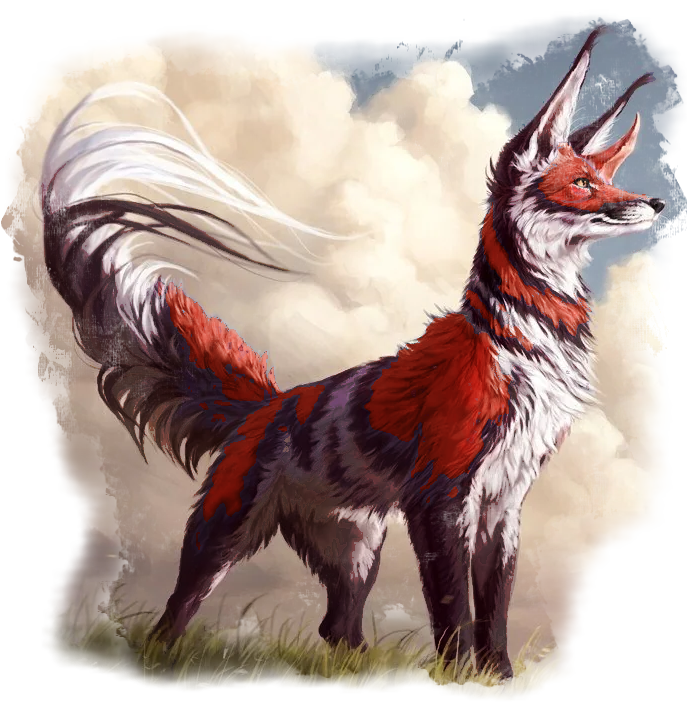
\includegraphics[width=0.65\columnwidth, height=155pt, keepaspectratio]{Monsters/Zircon_Fox.png}
\end{tabular}